\documentclass{cernrep}
\begin{document}
\title{PF hadron calibration}
\author{Changgi Huh}
\institute{Kyungpook National University, Republic of Korea}

\maketitle

Code description of PF hadron calibration.
Running with "root calibChris.C"

\section{functions}

The main function of this code is calibChris(). Inside of calibChris(), some functions and classes are used. The function list is 
\begin{itemize}
\item InitBarrelAlpha()
\item LoadOldThresholds()
\item getValuesFromTree(vector<double>\&, vector<double>\&, vector<double>\&, vector<double>\&, vector<double>\&)
\item GetETrueBin(double)
\item GetETrueBinEta(double)
\item assignvalues(vector<float>*, vector<float>*, vector<float>*, vector<float>*)
\item drawCompare(TGraph\&, TGraph\&, TGraph\&, TGraph\&)
\item drawEtaDependence(TH2F*, TGraph*)
\item drawGausFit(TH2F*, TGraph*, TGraph*, TString)
\end{itemize}

The class list is

\begin{itemize}
\item ABC
\item AlphaBeta
\end{itemize}

Inside of two classes, several functions are exist. The lists are in the Figure \ref{ABC} and Figure \ref{AlphaBeta}. Detail descriptions are written in below.

\begin{figure}[ht]
%\begin{center}
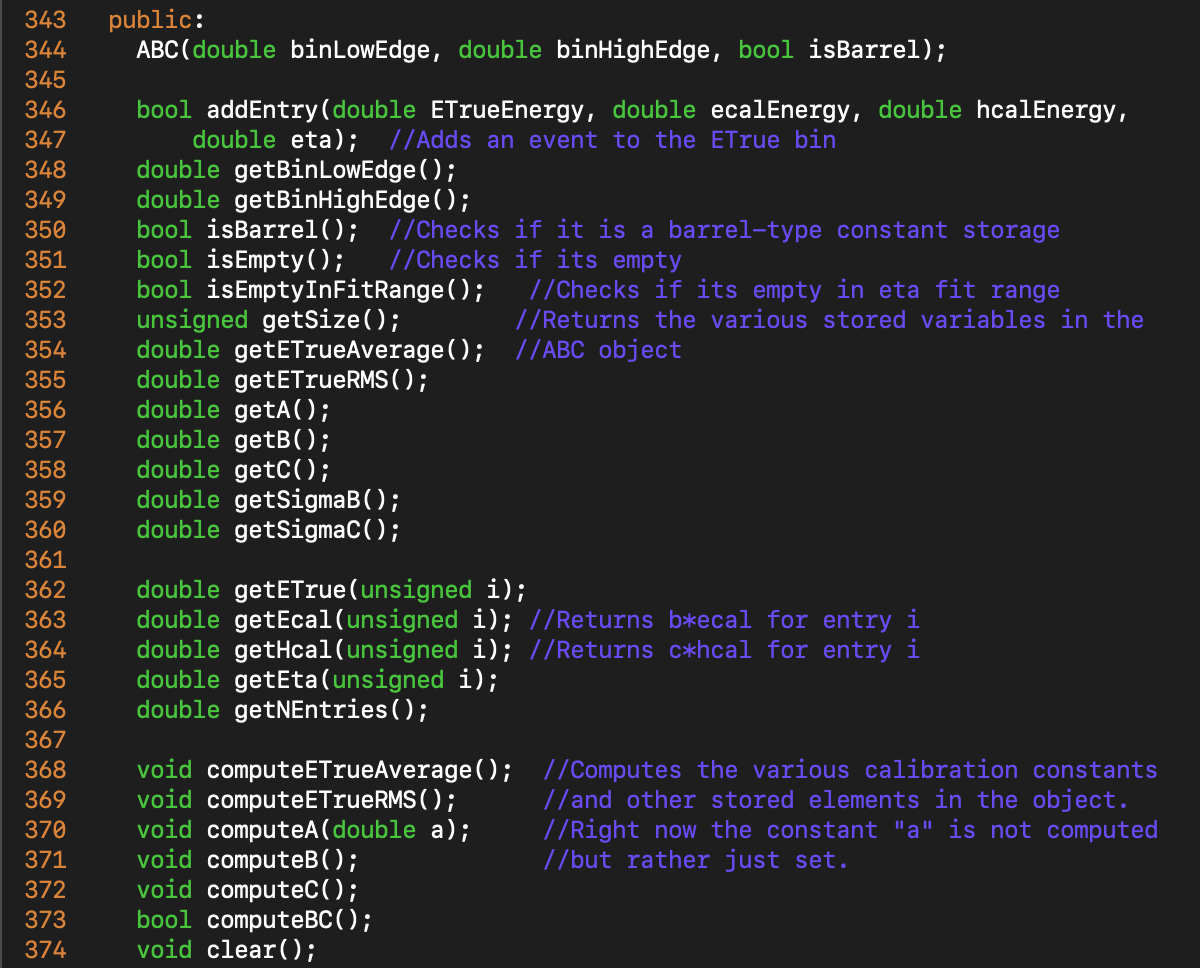
\includegraphics[width=1.0\textwidth]{fig/ABC.png}
\caption{functions in ABC class}
\label{ABC}
%\end{center}
\end{figure}

\begin{figure}[ht]
%\begin{center}
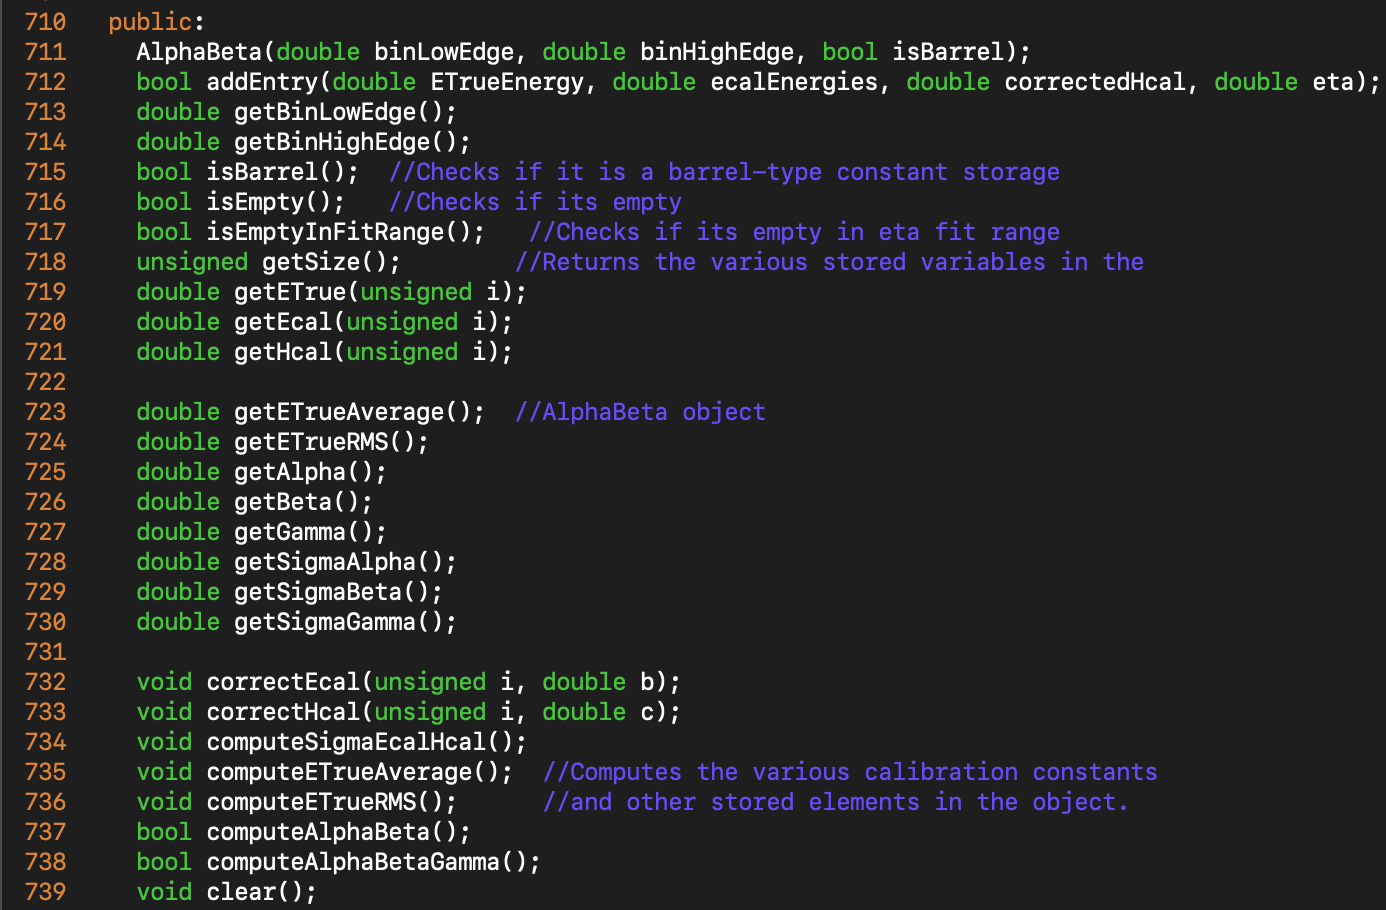
\includegraphics[width=1.0\textwidth]{fig/AlphaBeta.png}
\caption{functions in AlphaBeta class}
\label{AlphaBeta}
%\end{center}
\end{figure}

\subsection{functions}

\subsubsection{InitBarrelAlpha}

It initialize some TF1 type functions. Initialized functions don't use anymore.

\subsubsection {LoadOldThresholds}

Load thereshold values that comes from Shubham who did offline PF hadron calibration. 3.5 is used for EH hadrons and 2.5 is used for H hadrons. Don't foucs on the "old". This value used for Run2 data taking.

\subsubsection {getValuesFromTree}
This function open the ntuples and get value from ntuples. Get generator level information(energy, eta and phi) and get particle flow based information(momentum, id, eta, phi, measured energy in ECAL and HCAL)


\subsubsection {GetETrueBin}

It made bin of true energy for energy calibration.

\subsubsection {GetETrueBinEta}

It made bin of true energy for eta-energy calibration.

\subsubsection {assignvalues}

This is unused function.

\subsubsection {drawCompare}

This is unused function.

\subsubsection {drawEtaDependence}

Draw eta dependent plot. It is Figure \ref{EtaDependent}.

\begin{figure}[ht]
%\begin{center}
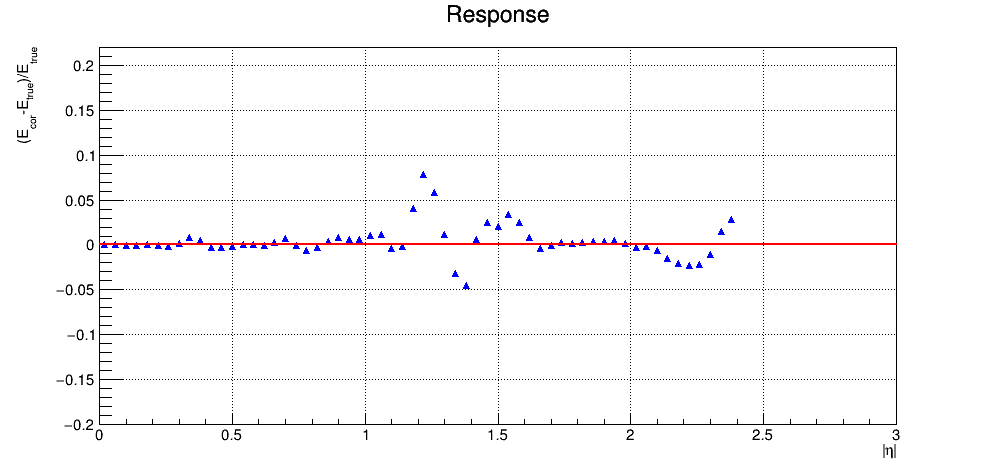
\includegraphics[width=1.0\textwidth]{fig/corrEtaDependenceEH_JME_GT_sample.png}
\caption{eta dependent response result.}
\label{EtaDependent}
%\end{center}
\end{figure}

\subsubsection {drawGausFit}

Fit the $\frac{E_{True}-E_{Measure}}{E_{True}}$ distribution  using Gaussian distribution. The mean from fitted Gaussian distribution refer to response distribution and sigma from  fitted Gaussian distribution refer to resolution distribution. The full resolution distribution is fitted by $\sqrt{A^2+\frac{B^2}{x}*\frac{C^2}{x^2}}$. //
To check the calibration is worked, response distribution is gone to 0.

\subsection{classes}

To calibrate energy, made two different classes, ABC and AlphaBeta. ABC is energy dependent calibration and AlphaBeta is eta dependent calibration.

\subsubsection{ABC}

ABC is energy dependent calibration.

\subsubsubsection{construct class}

When ABC class is constructed, lower and upper energy bin edge and barrel check parameter is inputted. Eta fit range is determined.

\subsubsubsection{addEntry}

If values are satisfied the selection, true energy, stored energy in ECAL and HCAL, eta and sigmaEcalHcal are saved in vectors. Those are used when calculate calibration constant.

\subsubsubsection{getBinLowEdge}

This is unused function.

\subsubsubsection{getBinHighEdge}

This is unused function.

\subsubsubsection{isBarrel}

This is unused function.

\subsubsubsection{isEmpty}

If true energy value is exist, it return true.

\subsubsubsection{isEmptyInFitRange}

If eta is satisfied eta selection, it return true.

\subsubsubsection{getSize}

It returns size of true energy.

\subsubsubsection{getETrueAverage}

It returns average of true energy.

\subsubsubsection{getETrueRMS}

It returns RMS of true energy.

\subsubsubsection{getA}

It return threshold. 3.5 GeV for EH hadron, 2.5 GeV for H hadron.

\subsubsubsection{getB}

It returns calibration constant A for EH hadrons.

\subsubsubsection{getC}

It returns calibration constant B for EH hadrons.

\subsubsubsection{getSigmaB}

It returns sigma of calibration constant A for EH hadrons.

\subsubsubsection{getSigmaC}

It returns sigma of calibration constant B for EH hadrons.

\subsubsubsection{getETrue}

It returns true energy.

\subsubsubsection{getEcal}

It returns measured energy in ECAL.

\subsubsubsection{getHcal}

It returns measured energy in HCAL.

\subsubsubsection{getEta}

It returns eta.

\subsubsubsection{getNEntries}

It returns size of true energies.

\subsubsubsection{computeETrueAverage}

Calculate average of true energy.

\subsubsubsection{computeETrueRMS}

Calculate RMS of true energy.

\subsubsubsection{computeA}

It return threshold. 3.5 GeV for EH hadron, 2.5 GeV for H hadron.

\subsubsubsection{computeB}

Calculate energy calibration constant A and sigma of A for EH hadrons.

\subsubsubsection{computeC}

Calculate energy calibration constant B and sigma of B for EH hadrons.

\subsubsubsection{computeBC}

Calculate energy calibration constant C and sigma of C for H hadrons.

\subsubsubsection{clear}

Delete values.

\subsubsection{AlphaBeta}

AlphaBeta is eta dependent calibration.

\subsubsubsection{construct class}

When AlphaBeta class is constructed, lower and upper energy bin edge and barrel check parameter is inputted. Eta fit range is determined.

\subsubsubsection{addEntry}

If values are satisfied the selection, true energy, stored energy in ECAL and HCAL, eta and threshold are saved in vectors. Those are used when calculate calibration constant.

\subsubsubsection{getBinLowEdge}

This is unused function.

\subsubsubsection{getBinHighEdge}

This is unused function.

\subsubsubsection{isBarrel}

This is unused function.

\subsubsubsection{isEmpty}

If true energy value is exist, it return true.

\subsubsubsection{isEmptyInFitRange}

If eta is satisfied eta selection, it return true.

\subsubsubsection{getSize}

It returns size of true energy.

\subsubsubsection{getETrue}

It returns true energy.

\subsubsubsection{getEcal}

It returns measured energy in ECAL.

\subsubsubsection{getHcal}

It returns measured energy in HCAL.

\subsubsubsection{getETrueAverage}

It returns average of true energy.

\subsubsubsection{getETrueRMS}

It returns RMS of true energy.

\subsubsubsection{getAlpha}

It returns calibration constant Alpha.

\subsubsubsection{getBeta}

It returns calibration constant Beta.

\subsubsubsection{getGamma}

It returns calibration constant Gamma. This is unused function.

\subsubsubsection{getSigmaAlpha}

It returns sigma of calibration constant Alpha.

\subsubsubsection{getSigmaBeta}

It returns sigma of calibration constant Beta.

\subsubsubsection{getSigmaGamma}

It returns sigma of calibration constant Gamma. This is unused function.

\subsubsubsection{correctEcal}

It correct measured energy in ECAL using calibration constant.

\subsubsubsection{correctHcal}

It correct measured energy in HCAL using calibration constant.

\subsubsubsection{computeSigmaEcalHcal}

It compute sigma of correct measured energy in HCAL using calibration constant.

\subsubsubsection{computeETrueAverage}

Calculate average of true energy.

\subsubsubsection{computeETrueRMS}

Calculate RMS of true energy.

\subsubsubsection{computeAlphaBeta}

Calculate eta dependent calibration constant Alpha and Beta.

\subsubsubsection{computeAlphaBetaGamma}

This is unused function.

\subsubsubsection{clear}

Delete values.

\end{document}
